\documentclass[border=6pt]{standalone}
\usepackage{amsmath}
\usepackage{tikz}
\usetikzlibrary{arrows.meta,decorations.pathmorphing}
\begin{document}
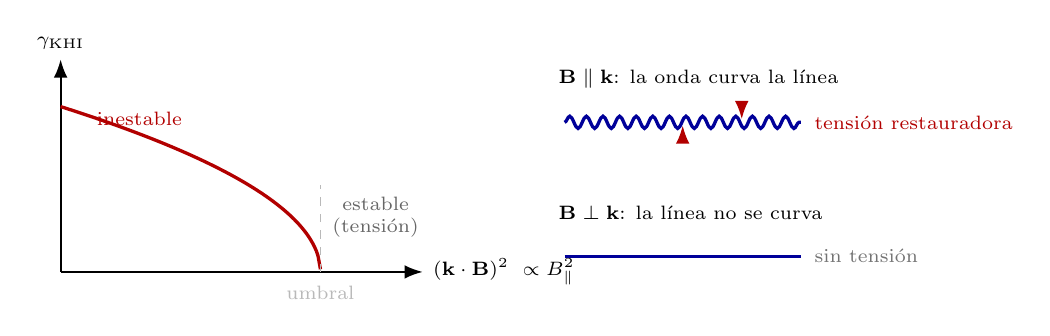
\begin{tikzpicture}[>=Latex,scale=1.0]

% ===== curva gamma vs (k.B)^2 =====
\begin{scope}
 \draw[->,thick] (0,0) -- (4.6,0) node[right,font=\scriptsize]{$(\mathbf k\cdot\mathbf B)^2\ \propto B_\parallel^2$};
 \draw[->,thick] (0,0) -- (0,2.7) node[above,font=\scriptsize]{$\gamma_{\rm KHI}$};
 \draw[red!70!black,very thick,smooth,samples=100,domain=0:3.3]
   plot (\x,{2.1*sqrt(max(0,1-(\x/3.3))});
 \draw[gray!55,dashed] (3.3,0) -- (3.3,1.1);
 \node[font=\scriptsize,gray!55,anchor=north] at (3.3,-0.05) {umbral};
 \node[font=\scriptsize,red!70!black] at (1.0,1.95) {inestable};
 \node[font=\scriptsize,black!60,align=center] at (4.0,0.7) {estable\\(tensi\'on)};
\end{scope}

% ===== insets: B paralela (tension) vs B perpendicular (sin tension) =====
\begin{scope}[xshift=6.4cm,yshift=1.5cm]
 \node[font=\scriptsize,anchor=west] at (-0.2,0.95) {$\mathbf B \parallel \mathbf k$: la onda curva la l\'inea};
 % linea de campo ondulada (estirada por la perturbacion)
 \draw[blue!60!black,very thick,decorate,decoration={snake,amplitude=2.2pt,segment length=6pt}]
   (0,0.4) -- (3.0,0.4);
 \draw[->,red!70!black,thick] (1.5,0.18) -- (1.5,0.36);
 \draw[->,red!70!black,thick] (2.25,0.62) -- (2.25,0.44);
 \node[font=\scriptsize,red!70!black,anchor=west] at (3.05,0.4) {tensi\'on restauradora};
\end{scope}
\begin{scope}[xshift=6.4cm,yshift=-0.2cm]
 \node[font=\scriptsize,anchor=west] at (-0.2,0.95) {$\mathbf B \perp \mathbf k$: la l\'inea no se curva};
 \draw[blue!60!black,very thick] (0,0.4) -- (3.0,0.4);
 \node[font=\scriptsize,black!55,anchor=west] at (3.05,0.4) {sin tensi\'on};
\end{scope}

\end{tikzpicture}
\end{document}
